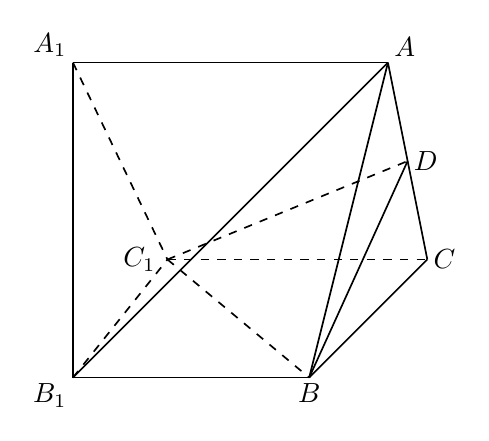
\begin{tikzpicture}[x=1cm,y=1cm,line width=.6pt,font=\normalsize,
  geometry edge/.style={solid,line width=.6pt},
  geometry label/.style={font=\normalsize,inner sep=2pt}]
\coordinate (Aone) at (0,4);
\coordinate (A) at (4,4);
\coordinate (Bone) at (0,0);
\coordinate (B) at (3,0);
\coordinate (Cone) at (1.2,1.5);
\coordinate (C) at (4.5,1.5);
\coordinate (D) at (4.25,2.75);
% top edge
\draw[geometry edge] (Aone)--(A);
% left lateral and bottom
\draw[geometry edge] (Aone)--(Bone);
\draw[geometry edge] (Bone)--(B);
% prism diagonals through C1
\draw[geometry edge] (Bone)--(A);
\draw[geometry edge] (A)--(B);
\draw[geometry edge] (A)--(D);
\draw[geometry edge] (D)--(C);
\draw[geometry edge] (D)--(B);
\draw[geometry edge] (B)--(C);
% hidden edges meeting at C1
\draw[geometry edge,dashed] (Aone)--(Cone);
\draw[geometry edge,dashed] (Bone)--(Cone);
\draw[geometry edge,dashed] (Cone)--(C);
\draw[geometry edge,dashed] (Cone)--(D);
\draw[geometry edge,dashed] (Cone)--(B);
\node[geometry label,above left] at (Aone) {$A_{1}$};
\node[geometry label,above right] at (A) {$A$};
\node[geometry label,below left] at (Bone) {$B_{1}$};
\node[geometry label,below] at (B) {$B$};
\node[geometry label,left,xshift=-2pt] at (Cone) {$C_{1}$};\node[geometry label,right] at (C) {$C$};
\node[geometry label,right] at (D) {$D$};
\end{tikzpicture}
